\documentclass[11pt,a4paper,twoside]{article}
\usepackage{tascar}
\pagenumbering{arabic}
\pagestyle{empty}
\showtutorialtrue
\begin{document}
\setcounter{tutorial}{4}
\begin{tutorial}{Audio-visual interaction}{Seminar room, VR-Lab}
  Create the game ``Dungeons of screams'' to design an interactive
  audio-visual detection experiment with \tascar{} and the blender game engine.

\begin{learnitems}
\item How to send position and orientation of objects to a game engine
\item How to control \tascar{} properties from a game engine
\item How to use navigation meshes and game controllers in \tascar{}
\end{learnitems}

\begin{appitems}
\item Audio-visual environments for hearing aid research
\item Game programming \& having fun
\end{appitems}

~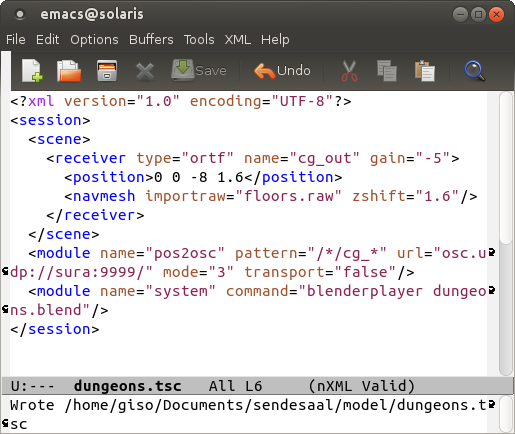
\includegraphics[height=0.36\columnwidth]{t5_dungeonstsc.png}\hfill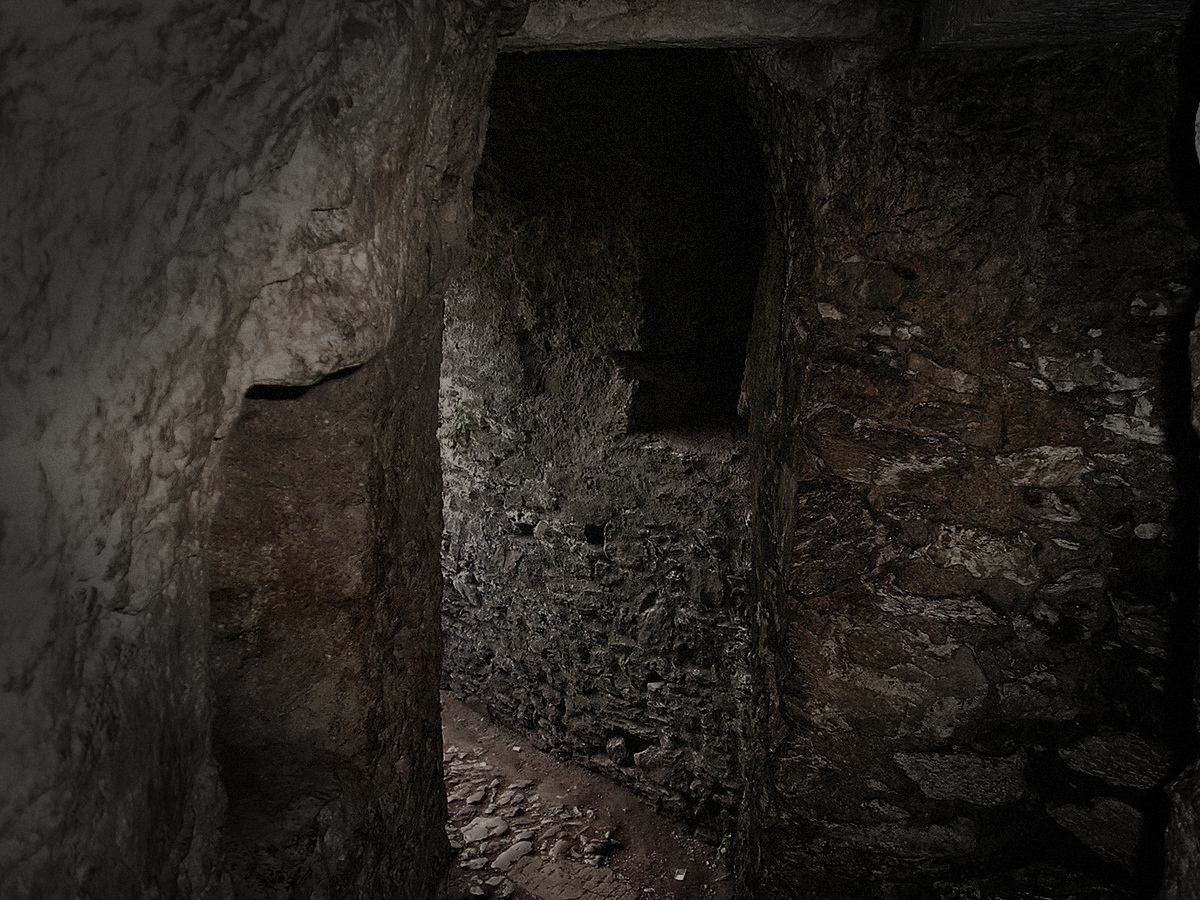
\includegraphics[height=0.36\columnwidth]{dungeons.jpg}~

\end{tutorial}

\ifshowtutorial

\newpage

\subsection*{The Story}

Good old OLSA was caught and locked into the dungeon of screams. Find
the OLSA and free it! Stop the other voices!

\subsection*{How to do it}

The game is split into two processes: TASCAR will control the audio as
well as the motion of objects. The blender game engine
(\url{http://www.blender.org/}) will render the visual components and
its Python interface can be used for the game logic.

Open your dungeon graphical environment with blender:
\begin{verbatim}
blender dungeon.blend &
\end{verbatim}
Switch between ``Default'' view, ``Game logic'' view and ``Scripting''
view. We use blender logic bricks only for running our main Python
script \verb!main.py! -- in that script we do all the logic, e.g.,
receiving and sending of OSC messages.

Look at the TASCAR file \verb!tutorial5.tsc!. It looks like a mess --
the first scene defines the main acoustic environment. Add some real
screams to the ``scream'' object. You can record them in the gesture
lab (ask for help if needed).

Out target is the ghost of OLSA. It is following a track defined in
blender. See below how to change the path. We also have a door source,
which will be triggered when we approach it.  The walls of the room
are also defined in blender.  Our receiver is controlled by a game
controller, but should always be linked to a navigation mesh. A second
receiver (omni-directional) is used to generate the diffuse
reverberation.

Most important part for the interaction between TASCAR and the blender
game engine are the modules defined at the end of the session file:
\begin{lstinputlisting}[language=tsc,caption={},linerange=51-71,firstnumber=51]{../examples/tutorial5_audiovisual/tutorial5.tsc}
\end{lstinputlisting}
The module \verb!pos2osc! can track TASCAR objects and send their
positions to the game engine.

The \verb!nearsensor! can detect when we are close to objects, and can
trigger user defined OSC messages.

Animations in TASCAR are created using the \verb!motionpath!
module. These animations can be triggered via OSC (see line 54).

Game controllers are connected with the \verb!joystick! module. Axis
events are interpreted to control the receivers, and all events can be
sent also via OSC, to trigger actions in the game engine.

\subsection*{Create/update paths and meshes for use in TASCAR scenes}

Motion paths (in form of a CSV file) and face groups (text file with
vertex positions) can be exported from blender. If you would like to
export something, put it into the ``tascar'' scene of your blend file
(switch back to ``game'' scene before saving the blend file, otherwise
the game will not work).

Modify your paths, reflector and navigation mesh to your needs. Keep
it simple. To re-export to TASCAR, type
\begin{verbatim}
blender -b dungeon.blend -P export_mesh.py
\end{verbatim}


\subsection*{The main action: Free OLSA}

To free the OLSA, create a near sensor, and trigger an action in the
game engine. For example, a button will be active only if you are near
the target. If you trigger the button near a scream, you might kill
it. Figure out yourself! See the end of \verb!main.py! for an example.

\fi
\end{document}
%%  LocalWords:  OSC TASCAR
